\documentclass[a4paper, 12pt]{article}
\usepackage{cmap}           % Пакет для поиска в полученной пдфке
\usepackage[utf8]{inputenc} % Ззамена кодировки файла на utf8
\usepackage[T2A]{fontenc}   % Подключение кодировки шрифтов
\usepackage[russian]{babel} % Использование русского языка 
\usepackage[left=2cm, right=2cm, top=1cm, bottom=2cm]{geometry} % Изменение размеров полей
\usepackage{indentfirst}    % Красная строка в начале текста
\usepackage{amsmath, amsfonts, amsthm, mathtools, amssymb, icomma, units, yfonts}
\usepackage{amsthm} % Пакет для нормального оформления теорем
\usepackage{graphicx}
\usepackage{tikz}
\usepackage{esvect}
\usepackage{enumitem}
\usetikzlibrary{calc,matrix}

%Теоремы
%11.01.2016
\newtheorem*{standartbase}{Теорема о стандартном базисе}
\newtheorem*{fulllemma}{Лемма}
\newtheorem*{sl1}{Следствие 1}
\newtheorem*{sl2}{Следствие 2}
\newtheorem*{monotonousbase}{Теорема о монотонном базисе}
\newtheorem*{scheme}{Утверждение 1}
\newtheorem*{n2}{Утверждение 2}
\newtheorem*{zhegalkin}{Теорема Жегалкина}
\newtheorem*{poste}{Теорема Поста}
\newtheorem*{cantor}{Теорема Кантора}
\newtheorem*{cantorfull}{Полная теорема Кантора}
\newtheorem*{cantorbern}{Теорема Кантора-Бернштейна}

%18.01.2016
\newtheorem*{on2n}{Теорема}
\newtheorem*{o2ndivn}{Теорема}
\newtheorem*{existsFgthen2ndivn}{Теорема}

\renewcommand{\qedsymbol}{\textbf{Q.E.D.}}
\newcommand{\definition}{\underline{Определение:} }
\newcommand{\statement}{\underline{Утверждение:} }
\newcommand{\note}{\underline{Замечание:} }

\newcommand{\Z}{\mathbb{Z}}
\newcommand{\N}{\mathbb{N}}
\newcommand{\Q}{\mathbb{Q}}
\newcommand{\R}{\mathbb{R}}



\begin{document}
\title{Дискретная математика. Модуль 3. Лекция 4}
\author{Лекторий ПМИ ФКН 2015-2016\\Гринберг Вадим\\Жижин Пётр\\Пузырев Дмитрий}
\date{1 февраля 2016}

\maketitle
\section{Равномощность некоторых множеств}
\subsection*{Множество двоичных слов. Множество пар натуральных чисел. Множество конечных последовательностей натуральных чисел}

Рассмотрим следующие множества:

\begin{itemize}
        \item $\{ 0, 1\}^*$ -- множество двоичных слов.
        \item $\N$ -- множество натуральных чисел (целые положительные и 0).
        \item $\N \times \N$ -- множество пар натуральных чисел.
        \item $\N^*$ -- множество конечных последовательностей натуральных чисел.
\end{itemize}

Докажем, что между ними есть эффективная биекция (то есть задаваемая простым алгоритмом).

\statement $\{ 0, 1\}^* \sim \N$.
\begin{proof}

    Рассмотрим такую функцию $f: W \to \overline{1W_{2}} - 1$, действующую из множества двоичных чисел в множество чисел, полученных путём вычитания единицы из значения двоичной записи исходного числа с приписанной вначале единицей. Тогда мы сопоставим каждому двоичному числу некоторое натуральное.
    
    \begin{itemize}
        \item $\{\ \} \to \overline{1_{2}} - 1 = 0$
        \item $0 \to \overline{10_{2}} - 1 = 1$
        \item $1 \to \overline{11_{2}} - 1 = 2$
    \end{itemize}
    
    Докажем, что это отображение -- биекция.
    
    \textbf{Инъективность}
    
        Пусть у двух двоичных слов совпали образы, то есть им соответствует одно и то же натуральное число. Прибавим к этому числу единицу, получив тем самым число вида $\overline{1W_{2}}$. Но тогда по числу $W_{2}$ мы однозначно восстановим исходное слово, следовательно, изначальные двоичные слова равны.
        
    \textbf{Сюръективность}
    
        Возьмём любое число $P \in Z_{+}$, тогда $P$ представимо в виде $\overline{1W_{2}}$ для некоторого $W$. У получившегося числа $\overline{1W_{2}}$ старшая цифра обязательно единица, тогда само число $W$ есть единственный прообраз числа $P = \overline{1W_{2}}$ по построению.
    
\end{proof}

\statement $\N \times \N \sim \N$.
\begin{proof}

    Есть 2 варианта построить биекцию между этими двумя множествами: первый -- диагональный метод, рассмотренный ранее. Тогда:
    $(x, y) \to \dbinom {x + y - 1}2 + y$.
    
    Рассмотрим второй вариант:
    
    Построим биекцию $\N \times \N \to \Z_{+}$, а так как $\Z_{+} \sim \N$, то мы тем самым докажем треубемое.
    
    Пусть $f : (x, y) \to 2^x(2y + 1)$ -- функция из множества пар в множество целых чисел, представленных в следующем виде. Покажем, что это -- биекция.
    
    \textbf{Сюръективность}
    
        По Основной Теореме Арифметики, любое целое положительное число представимо в виде произведения степеней его простых множителей:
        
        $\Z_{+} = 2^{\alpha_2} \cdot 3^{\alpha_3} \cdot \ldots \cdot p^{\alpha_p} \Rightarrow$ вынесем степень двойки. Оставшееся число $3^{\alpha_3} \cdot \ldots \cdot p^{\alpha_p}$ -- нечётное, значит, представимо в виде $2y + 1$ для некоего числа $y$.
        
        Тогда этому значению нашей функции будет соответствовать пара чисел $\alpha_{2}$ и $y$: $f(\alpha_{2}, y) = 2^{\alpha_{2}}(2y + 1) = z$, где $z \in \Z_{+}$. 
        
        Следовательно, для любой пары чисел $(x, y)$ существует число вида $2^x(2y + 1)$.
        
    \textbf{Инъективность}
    
        По Основной Теореме Арифметики разложение целого положительного числа является единственным.
        
        Отсюда следует, что разложение вида  $\Z_{+} = 2^{\alpha_2} \cdot 3^{\alpha_3} \cdot \ldots \cdot p^{\alpha_p}$, определяется единственным образом $\Rightarrow$ соответствующее этому разложению число $2^x(2y + 1)$ определяется единственным образом $\Rightarrow$ любой паре $(x, y)$ будет соответствовать только одно число вида $2^x(2y + 1)$ и инъективность выполнена.
\end{proof}

\statement $\N^* \sim \N$.
\begin{proof}

    Построим биекцию $\N^*  \to \Z_{+}$, а так как $\Z_{+} \sim \N$, то мы тем самым докажем треубемое.
    
    Пусть $f : (x_1, x_2, \ldots , x_n) \to p_{1}^{x_1} \cdot p_{2}^{x_2} \cdot \ldots \cdot p_{n}^{x_n + 1}$ -- функция из множества последовательностей натуральных чисел в целые положительные числа, представленные в виде произведения степеней некоторых различных простых чисел. Покажем, что это -- биекция.
    
    \textbf{Инъективность}
        
        Предположим, что две последовательности задают одно и то же число. Тогда, выписывая показатели степеней числа, восстанавливаем две исходные последовательности. По ОТА любое натуральное  число однозначно представимо в виде произведения степеней простых сомножителей, значит, получившиеся последовательности равны.
        
        Здесь же приведём ответ, почему степень числа $p_n$ равна $x_n + 1$. Если бы показатель степени был равен $x_n$, то, к примеру, последовательности $\{1, 0\}$ и $\{1, 0, 0\}$ задавали бы одно и то же число: $2^1 \cdot 3^0 = 2^1 \cdot 3^0 \cdot 4^0$ -- инъективность бы не соблюдалась.
        
    \textbf{Сюръективность}
    
        Основная Теорема Арифметики гарантирует существование для любого натурального числа разложения в виде произведения степеней простых сомножитилей. Значит, любому набору $f : (x_1, x_2, \ldots , x_n)$ можно сопоставить такое разложение, поэтому сюръекция установлена.
        

\end{proof}

\subsection*{Множество всех подмножеств $\N$. Множество последовательностей натуральных чисел. Множество действительных чисел}

    Рассмотрим следующие множества:

    \begin{itemize}
        \item $\Phi(\N)$ -- множество всех подмножеств $\N$.
        \item $2^{\N}$ -- множество последовательностей натуральных чисел.
        \item $\R$ -- множество действительных чисел.
    \end{itemize}

    Определим действительные числа следующим образом: сопоставим каждому $x \in \R$ двоичное число: $\pm \lefteqn{\underbrace{\phantom{10110 \dots 1011}}_{\text{целая часть}}}10110 \dots 1011 .\overbrace{110001 \dots 00110}^{\text{дробная часть}}$. Считаем известным, что ряд из каких-то степеней двоек сходится, причём запрещаем в числах данного вида "хвосты из единиц".

\statement $\Phi(\N) \sim 2^{\N}$.
\begin{proof}
    Введём функцию $f: \N \to \chi(x)$ -- индикаторная функция $=$
    $\begin{cases}
            1, \  x \in \N\\
            0, \ x \notin \N
    \end{cases}$
    
    То есть, для каждого подмножества множества $\phi(\N)$ выписываем в ряд все натуральные числа, затем записываем для каждого натурального числа $1$, если оно входит в это подмножество, и $0$ иначе. Покажем, что это -- биекция.
    
    \textbf{Инъективность}
        
       Пусть у двух элементов $\N$ совпали образы. Тогда возьмём такое подмножество $\N^{'}$, в котором значение $f(\N^{'}) = 1$. Но тогда для каких-то $x_{i}, \  x_{j} \in f(\N^{'}) \ | \ x_{i} \neq x_{j}$ либо $x_{i} = 1, \  x_{j} = 0$, либо $x_{i} = 0, \  x_{j} = 1$. Следовательно, образы у этих двух элементов различны.
        
    \textbf{Сюръективность}
    
        Берём множество $\chi(x)$ и построим по нему элементы последовательности. Пусть мы получили 2 разных последовательности из одного двоичного числа. Но это означает, что в каком-то разряде двоичного числа не совпали цифры (в одном $0$, в другом $1$). Но тогда по построению это 2 разных числа.

\end{proof}
    
\statement $\R \sim 2^{\N}$.
\begin{proof}
    
    Из курса математического анализа был известнен факт, что $\R \sim (0, 1)$. Пусть $X$ -- множество последовательностей из $0$ и $1$ без хвостов из единиц. Тогда по определению существует биекция $X \leftrightarrow [0, 1)$.
    
    По определению $\R$: $[0, 1) \sim \pm 101 \ldots 001.1100 \ldots 01110$, тогда $X = 2^{\N} \backslash Y$, где $Y$ -- последовательность нулей и единиц с одиними единицами в конце.
    
    Из семинарских занятий нам известна теорема: если множество $A$ -- бесконечно, множество $B$ -- счётно, то $A \cup B \sim A$.
    
    Докажем, что множество $Y$ счётно. Пусть у нас есть какое-то число с одними единицами в конце: $w_{2}.1100110111111$ ($w_{2}$ -- целая часть числа). Если его инвертировать, то после точки получим двоичное число с бесконечным числом нулей в конце, единиц же будет счётное количество: $w_{2}.0011001000000$. Значит, эта новая последовательность нулей и единиц представляет какое-то натуральное число. Таким образом, мы построили биекцию $Y \leftrightarrow N$, значит по определению $Y$ счётно.
    
    Но тогда по теореме выше $2^{\N} = X \cup Y \sim X$, а так как $X \sim [0, 1)$, то $2^{\N} \sim [0, 1)$. 
    
    Очевидно, что множество $[0, 1] \sim [0, 1)$ -- то же множество без одной точки. Но тогда аналогично $[0, 1) \sim (0, 1) \sim \R$.
    
\end{proof}

\definition Вышеперечисленные множества принято называть \textit{континуальными}. Будем говорить, что множество $X$ имеет мощность континуум, если $X \sim \R$.

\subsection*{Теорема Кантора для натуральных чисел. Полная теорема Кантора. Теорема Кантора-Бернштейна}
    
\begin{cantor}
    $\N \nsim \R$
\end{cantor}

\begin{proof}

    Если вспомнить лекции по математическому анализу, мы доказывали неравномощность $\N$ и $(0, 1)$, воспользовавшись тем, что $\R \sim (0, 1)$.

    В этот раз воспользуемся $\R \sim 2^{\N}$, и докажем $\N \nsim 2^{\N}$ для получения требуемого.
    
    Докажем при помощи диагонального рассудения:
    
    Пусть $F = \{f_0, f_1, \ldots , f_n, \ldots \}$ -- множество последовательностей $f \in 2^{\N}$. Покажем, что $\exists x \in 2^{\N} : x \notin F$, тем самым доказав, что отображение $\N \to 2^{\N}$ не сюръективно.
    
    Запишем элементы $F$ в квадратную таблицу по правилу $f_i = \{f_{i0} \ f_{i1} \ldots f_{in}\}$:
    
    $\begin{array}{lcccr}
        f_0 = & f_{00} & f_{01} & \ldots & f_{0n}\\
        f_1 = & f_{10} & f_{11} & \ldots & f_{1n}\\
        \vdots & \vdots & \vdots & \ddots & \vdots \\
        f_n = & f_{n0} & f_{n1} & \ldots & f_{nn}\\
    \end{array}$
    
    Выпишем последовательность по диагонали: $f_{*} = \{f_{00} \ f_{11} \ f_{22} \ldots f_{n n}\}$. Тогда пусть $x = \{\overline{f_{00}} \ \overline{f_{11}} \ldots \overline{f_{n n}}\}$. Тогда $x \neq f_{i} \  \forall i \in [0, n]$, так как $x_{j} = \overline{f_{j j}} \neq f_{j j} \ \forall j$. Значит, отображение не сюръективно.
    
    Таким образом, $\N \nsim 2^{\N}$, и так как $\R \sim 2^{\N}$, то $\N \nsim \R$.
        
\end{proof}
    
\begin{cantorfull}
    $X \nsim 2^{X} \ \forall \ $ множества $X$. Иначе говоря, любое множество не равномощно множеству своих подможеств: $X \nsim \phi(x)$.
\end{cantorfull}

\begin{proof}
    
    Пусть имеется функция $f: X \to \Phi(x)$, сопоставляющая каждому множеству $x$ его подмножество. Докажем, что эта фунция не является биекцией. Для этого достаточно показать, что не соблюдается сюръективность.
    
    Возьмём множество $F = \{x \  | \ x \notin f(x)\} \in X$ -- множество элементов, точно не принадлежащих образу функции $f$. Докажем, что нет такого $y$, что $f(y) = F$.
    
    Пусть $y \in F \Rightarrow f(y) = F$, но тогда по определению $y \notin f(y) = F$ -- противоречие.
    
    Пусть теперь $y \notin F \Rightarrow X \backslash F = \{x \ | \ x \in f(x)\}$, но тогда $y \in f(y) = F$ -- противоречие. 
    
    В итоге получаем, что $F \notin f(x)$, значит, отображение не сюръективно. Следовательно, биекции $f: X \leftrightarrow \phi(x)$ нет, и $X \nsim 2^{X} \ \forall \ $ множества $X$.


\end{proof}

\definition{Будем говорить, что множество $A$ не больше множества $B$ ($A \leq B$) тогда и только тогда, когда $\exists f: A \to B$ -- инъекция.}

\vspace{\baselineskip}
\definition{Будем говорить, что множество $A$ не меньше множества $B$ ($A \geq B$) тогда и только тогда, когда $\exists f: A \to B$ -- сюръекция.}

\vspace{\baselineskip}
\note{$A \leq B \Longleftrightarrow B \geq A$.}

\vspace{\baselineskip}
\statement{Пусть $A, B \neq \oslash$. Тогда если $\exists f: A \to B$ -- инъекция, то $\exists g: B \to A$ -- сюръекция, и наоборот.}

\begin{proof}
Пусть $f: A \to B$ -- инъекция. Возьмём функцию $y(x)$, такую, что

\[
    y(x) = \begin{cases}
        f^{-1}(x), \  x \in f(A) \\
        a_{0} \in A, \  x \notin f(A)
    \end{cases}
\]
 -- мы получили сюръекцию из инъекции.
 
 Обратно: пусть $f: B \to  A$ -- сюръекция. Возьмём некий элемент $a \in A$, тогда $f^{-1}(a) \neq \oslash$. Но тогда, взяв нашу функцию $y(x)$, получаем: $y(a) \in f^{-1}(a)$. А так как множества из разных $a$ не пересекаются, то получаем инъективность.

\end{proof}
    
\begin{cantorbern}
    Если множество $A$ равномощно некоторому подмножеству множества $B$, а $B$ равномощно некоторому подмножеству множества $A$, то множества $A$ и $B$ равномощны.
\end{cantorbern}

\begin{proof}
 
 
 Пусть A равномощно подмножеству $B_1$ множества $B$, а $B$ равномощно подмножеству $A_1$ множества $A$ (см. риc. 1). При взаимно однозначном соответствии между $B$ и $A_1$ подмножество $B_1 \subset B$ переходит в некоторое подмножество $A_2 \subset A_1$. При этом все три множества $A, B_1$ и $A_2$ равномощны, --- и нужно доказать, что они равномощны множеству $B$, или, что то же самое, $A_1$.
 
 \begin{figure}[h]
\begin{center}
\begin{minipage}[h]{0.4\linewidth}
 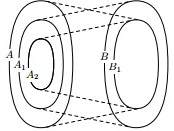
\includegraphics[height=5cm, width=\linewidth]{images/kantorbern1.jpg}
 \caption{Взаимные соответсвия между множествами}
 \end{minipage}
 \end{center}
 \end{figure}
 
 Теперь мы можем забыть про множество $B$ и его подмножества и доказывать такой факт:
 
 \textit{Если $A_2 \subset A_1 \subset A_0$ и $A_2 \sim A_0$, то все три множества
равномощны.}

 (Для единообразия мы пишем A0 вместо A.)
 
 Пусть $f$ — функция, осуществляющая взаимно однозначное соответствие $A_0 \rightarrow A_2$ (элемент $x \in A_0$ соответствует элементу $f(x) \in A_2$). Когда $A_0$ переходит в $A_2$, меньшее множество $A_1$ переходит в какое-то множество $A_3 \subset A_2$ (см. рис. 2). Аналогичным образом само $A_2$ переходит в некоторое множество $A_4 \subset A_2$. При этом $A_4 \subset A3$, так как $A_1 \subset A_2$.

 \begin{figure}[h]
\begin{center}
\begin{minipage}[h]{0.4\linewidth}
 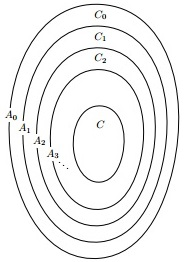
\includegraphics[height=5cm, width=\linewidth]{images/kantorbern2.jpg}
 \caption{Последовательные вхождения множеств}
 \end{minipage}
 \end{center}
 \end{figure}
 
 Продолжая эту конструкцию, мы получаем убывающую последовательность множеств
 
 \[A_0 \supset A_1 \supset A_2 \supset A_3 \supset A_4 \supset \ldots\]

 и взаимно однозначное соответствие $f : A_0 \rightarrow A_2$, при котором $A_i$ соответствует $A_{i + 2}$ (иногда это записывают так: $f(A_i) = A_{i+2}$). Формально можно описать $A_{2n}$ как множество тех элементов, которые получаются из какого-то элемента множества $A_0$ после $n$-кратного применения функции $f$. Аналогичным образом $A_{2n + 1}$ состоит из тех и только тех элементов, которые получаются из какого-то элемента множества $A_1$ после $n$-кратного применения функции $f$.
 
 Заметим, что пересечение всех множеств $A_i$ вполне может быть непусто: оно состоит из тех элементов, у которых можно сколько угодно раз брать $f$-прообраз. Теперь можно сказать так: множество $A_0$ мы разбили на непересекающиеся слои $C_i = A_i / A_{i+1}$ и на
сердцевину $C =\cap_i A_i$.

 Слои $C_0, C_2, C_4, \ldots$ равномощны (функция $f$ осуществляет взаимно однозначное соответствие между $C_0$ и $C_2$, между $C_2$ и $C_4$ и т.д.):

\[C_0 \xrightarrow{f} C_2 \xrightarrow{f} C_4 \xrightarrow{f} \ldots\]

То же самое можно сказать про слои с нечётными номерами:

\[C_1 \xrightarrow{f} C_3 \xrightarrow{f} C_5 \xrightarrow{f} \ldots\]

Можно ещё отметить (что, впрочем, не понадобится), что функция $f$ на множестве $C$ осуществляет его перестановку.

Теперь легко понять, как построить взаимно однозначное соответствие $g$ между $A_0$ и $A_1$. Пусть $x \in A_0$. Тогда соответствующий ему элемент $g(x)$ строится так: $g(x) = f(x)$ при $x \in C_{2k}$ и $g(x) = x$ при $x \in C_{2k + 1}$ или $x \in C$ (см. рис. 3)

\begin{figure}[h]
\begin{center}
\begin{minipage}[h]{0.4\linewidth}
 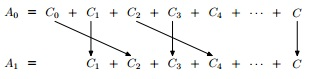
\includegraphics[height=2cm, width=\linewidth]{images/kantorbern3.jpg}
 \caption{Построение взаимно-однозначного соответствия}
 \end{minipage}
 \end{center}
 \end{figure}

\end{proof}
    
\end{document}